\section{Online Search}
In the preceeding section we showed that it is possible to break a large 
number of path symmetries by decomposing a 4-connected grid map into 
a set of empty rectangular rooms and pruning all nodes from the interior of
each room.
However, it is often the case that a pruned node might be required at a later
point as a start or goal location for an agent.
To solve this problem we propose to insert the start or goal (or both if necessary)
back into the graph for the duration of the search using the following procedure:
\begin{enumerate}
\item{If the start and goal are not in the same room, connect each of them
to the closest neighbours on each side of the perimeter of the empty room (see Figure \ref{fig-insertion}).}
\item{If the start and goal are in the same room no insertion is required;
 take the Manhattan distance between them as the length of the optimal path (see Figure \ref{fig-noinsertion}).}
\end{enumerate}
We claim that this procedure does not affect the optimality guarantees associated with traversing
across the room that the start or goal node is located in. 

\begin{figure}[t]
	\label{fig-roomtraversal}
	\vspace{-4pt}
       \begin{center}
           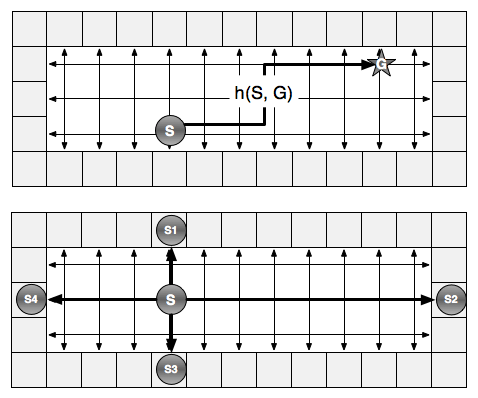
\includegraphics[scale=0.50, trim = 10mm 10mm 10mm 0mm]{diagrams/roomtraversal.png}
       \end{center}
	\vspace{-3pt}
       \caption{(Top) When $S$ and $G$ are in the empty room no insertion is necessary and we take the 
				Manhattan distance as the length of the optimal path.
				(Bottom) $S$ is a node previously pruned and $G$ is on the perimeter.
				We insert $S$ into the graph and connect it to neighbour on each side of the empty room.
				Then, an optimal-length path to $G$ can always be found.}
       \label{fig-ohacontrast}
	\vspace{-15pt}
\end{figure}

\begin{lemma}
\label{thm-insertion}
Let $R$ be an empty rectangular room and $N \in R$ the set of interior nodes.
For any pair of nodes $s, g \in R$ it is always possible to construct an optimal
length path which mentions only nodes in $\lbrace s, g \rbrace \bigcup  R \setminus N$.
\end{lemma}
\begin{proof}
First, suppose $g$ is a node on the perimeter of $R$ and $s \in N$ is an interior node that we 
have previously pruned (or vice versa).
We insert $s$ into the graph and connect it to 
$\lbrace s'_{1}, s'_{2}, s'_{3}, s'_{4} \rbrace \in R \setminus N$; the closest neighbours on 
each side of the perimeter.
The weight of each edge incident with $s$ is equal to the Manhattan distance between
$s$ and each $s'_{i}$.
To find an optimal path to $g$ we travel from $s$ to the the node $s'_{i}$ which is closest
to $g$. 
From there we travel along the perimeter of $R$ until we reach $g$.
\par
Next, suppose $s, g \in N$. 
In this case we do not insert anything; the length of the optimal path is equal
to the Manhattan distance between $s$ and $g$.
\end{proof}

Once the search has finished we remove the start and goal from the graph.
The time required in each case (insertion and deletion) is constant.
We claim that this procedure, together with Lemma \ref{thm-roomtraversal}, is sufficient to 
guarantee that A* will always return an optimal solution if one exists.

\begin{theorem}
For every optimal length path $\pi^*(s, g)$ in a 4-connected grid map there exists
an equivalent length path $\pi'(s, g)$ in the pruned version of the grid map.
\end{theorem}
\begin{proof}
Follows from Lemma \ref{thm-roomtraversal} and Lemma \ref{thm-insertion}.
For every optimal length segment of $\pi^{*}(s, g)$ which traverses
through an empty room there is an equivalent segment which mentions only nodes
on the perimeter of each room. 
Thus the length of $\pi'(s, g)$ is equal to the length of $\pi'(s,g)$.
\end{proof}

\begin{figure*}[t]
	\label{fig-contrast}
	\vspace{-4pt}
       \begin{center}
           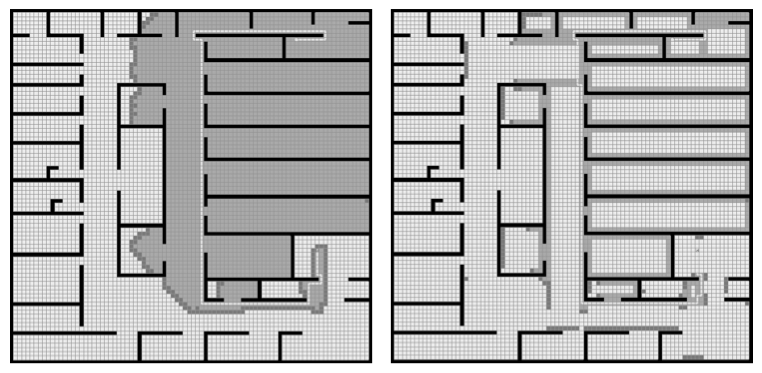
\includegraphics[scale=0.50, trim = 10mm 10mm 10mm 0mm]{diagrams/oha_contrast.png}
       \end{center}
	\vspace{-3pt}
       \caption{\textbf{(a)} A* solving a problem on a typical ($86\times88$) game map. 
Expanded nodes are marked light grey while nodes at the frontier of the search are dark grey.
\textbf{(b)} OHA* solving the same problem. A number of large rooms have been identified (not
all shown) and the algorithm only considers nodes along their perimeter.}
	\vspace{-15pt}
\end{figure*}

To highlight how effective our symmetry breaking technique can be in practice consider the example game map
in Figure \ref{fig-contrast}. 
The topography of this map is typical of what one might expect in a modern role-playing game
\footnote{Infact, most video game maps tend to be somewhat bigger than our example but for demonstration 
purposes it is quite sufficient.};
there are many rooms and corridors and many entrances to connect them.
Figure \ref{fig-contrast}(a) shows A* solving a typical problem on this map. 
In this case obtaining the optimal solution required expanding almost half the nodes in the state space.
Figure \ref{fig-contrast}(b) shows the same problem being solved by OHA*.
We were able to prune away large sections of the map by taking advantage of the fact that
such nodes never need to be expanded in order to retain optimality.
In this case OHA* expands less than $\frac{1}{3}$ of the area explored by A* and returns
a solution 4 times faster.

